\part{\textcolor{red}{Regelungstechnik}}
\section{Begrifflichkeiten}
	\begin{center}
		\begin{tabular}{l|p{12cm}}
			\textbf{Begriff} & \textbf{Beschreibung} 
			\\\hline & \\
			eingangsaffine Systeme & sind Systeme die in \textit{u} linear sind. Man sagt auch 		eingangslineare Systeme. \\& Genauer bedeutet es, dass sich die wirkende Stellgröße \textit{u} nur linear über die Zeit ändert.
			\\ & \\ \hline & \\
			relativer Grad $ \delta $ eines Systems & bei SISO-Sytemen gibt der relative Grad gleich dem Grad der Ableitungen der Ausgangsgröße $ y $ an, bei dem die $ \delta-$mal abgeleitete Ausgangsgröße erstmals direkt von der Stellgröße $ u $ abhängt: $ y^{(\delta)}_{i}=fcn(u) $. Ist der rel. Grad eines Systems \textit{wohldefiniert}, dann ist es Eingangs-/Ausgangs-linearisierbar. Für lineare Systeme entspricht der relative Grad dem Differenzgrad des Zähler- und Nennerpolynoms.  Der
			relative Grad r auch als die Anzahl der Integratoren gedeutet werden, die der Eingang u
			durchlaufen muss, bevor er den Ausgang y beeinflusst. In anderen Worten wird der Ausgang $ y^{(\delta)} $ direkt vom Eingang $ u $ beeinflusst und der Ausgang $ y $ erst über $ \delta $ Integratoren. Der relative Grad r ist somit ein Maß
			für die Mindestverzögerung im E/A-Verhalten.\\& [\textsc{Nichtlineare Systeme und Regelungen, Jürgen Adamy S290}]
			\\ & \\ \hline & \\
			Transitionsmatrix $ \bm{\Phi}(t) \label{transitionsmatrix} $& Die Transitionsmatrix  $ \bm{\Phi}(t) $ beschreibt den Übergang des Zustandsvektors $ \bm{x}(t) $	von seinem Anfangswert $ \bm{x}_{0} $ zu seinem Wert zum Zeitpunkt t.\\ & $\bm{x}(t) = \bm{\Phi}(t)\bm{x}_{0} +\int_{0}^{t}\bm{\Phi}(\tau -t)\bm{Bu}(\tau)d\tau $
			\\ & \\ \hline & \\
			Diffeomorphismus \label{diffeomorphismus} & Ist eine nichtlineare Zustandstransformation $ \bm{z} = \bm{q}(\bm{x}), \quad \bm{x} = \bm{q}^{-1}(\bm{z}) $ die stetig differenzierbar und eindeutig ist. Letzteres bedeutet, dass jedem $ \bm{x} $ kann genau ein $ \bm{z} $ zugeordnet werden und umgekehrt.
			\\ & \\ \hline & \\
			
			
			
		\end{tabular}
	\end{center}
\section{Eigenschaften von Systemen}
	\subsection{Flachheit}
		Ist ein System \textit{flach}, so können die dynamischen Gleichungen des Systems so umgeformt werden, dass sich Eingangs- und Zustandsgrößen anhand von Funktionen darstellen die nur von den Ausgangsgrößen und deren Ableitungen abhängig sind. Dadurch ist es möglich für einen gewünschten Ausgangsgrößenverlaufs die nötigen Eingangs- und Zustandsgrößenverläufe direkt anzugeben. \\\\
		\textit{Beispiel}:
		\begin{eqnarray} 
			\dot{x}_{1}&=& x_{2}\nonumber\\
			\dot{x}_{2}&=& -x_{1}-x_{2}+u\nonumber\\
			y&=&x_{1}\nonumber
		\end{eqnarray}
		Die Zustandsgrößen des Systems können als Funktionen der der Ausgangsgrößen dargestellt werden.
		\[\bm{x}=\begin{bmatrix}x_{1}\\x_{2}\end{bmatrix} = \begin{bmatrix}y\\\dot{y}\end{bmatrix} \]
		Ebenso der Eingangsvektor aus der mittleren Gleichung.
		\[u=\ddot{y}+\dot{y}+y\]
		Bei einem solchen System wird \textit{y} als \textbf{flacher Ausgang} bezeichnet. Dabei ist es nicht relevant ob dieser Ausgang tatsächlich existiert oder nur ausgedacht - \textit{fiktiv} ist. Existieren nur \textit{fiktive} flache Ausgänge müssen diese für den Entwurf einer Steuerung in den realen Ausgang umgerechnet werden.\\
		\begin{tcolorbox}[title=Definition: Flachheit]
			Für Systeme
			\[\bm{\dot{x}}=\bm{f(x,u)}, \quad \bm{x}\in \mathbb{R}^{n}, \bm{u}\in \mathbb{R}^{m}  \]
			mit $ m\leq n $ (weniger Eingangs- als Zustandsgrößen) für die sich keine Stellgröße $ u_{i} $ als Funktion anderer Stellgrößen $ u_{j\neq i} $ darstellen lässt
			\[rang\bigg(\dfrac{\partial\bm{f(x,u)}}{\partial\bm{u}}\bigg)=m, \]
			ist die \textit{Flachheit} folgendermaßen definiert:
			\tcblower
			Es heißt flach wenn ein realer oder fiktiver Ausgangsvektor	
			\[\bm{y} = \bm{h}(\bm{x,u,\dot{u},...,u}^{\alpha})\]
			existiert, so dass\\\\	
			\textit{(1) der Zustandsvektor $ \bm{x} $ als Funktion von $ \bm{y} $ und einer endlichen Anzahl $ \beta $ von Ableitungen von $ \bm{y} $}
			\[\bm{x} =\bm{\varPsi}_{1}(\bm{y,\dot{y},...,y}^{(\beta)}) \]
			\textit{dargestellt werden kann,}\\\\
			\textit{(2) der Eingangsvektor $ \bm{u} $ als Funktion}
			\[\bm{u} =\bm{\varPsi}_{2}(\bm{y,\dot{y},...,y}^{(\beta+1)}) \]
			\textit{darstellbar ist,}\\\\
			\textit{(3) für Ein- und Ausgangsvektor}
			\[dim(\bm{y}) = dim(\bm{u})\]
			gilt.
		\end{tcolorbox}	
	
	
\section{Systemtransformationen}
	\subsection{Zustandstransformation}
		Die Wahl der Zustandsgrößen eines Systems sind keinesfalls eindeutig. Mit Hilfe einer \textit{Zustandstransformation} kann ein System in eine neue Systemdarstellung mit neuen Zustandsgrößen transformiert werden.
		\subsubsection{Lineare Zustandstransformation}
			Durch eine \textit{reguläre Zustandstransformation} der Form
			\[\bm{x}(t) = \bm{Vz}(t)  \]
			mit der regulären Matrix $ \bm{V} $ (reguläre Matrix: invertierbare, quadratische Matrix) lässt sich ein \textit{Axbu-Modell} mit dem Zustand $ \bm{x}(t) $ in die Form
			\[\bm{\dot{z}} = \bm{V}^{-1}\bm{AVz} + \bm{V}^{-1}\bm{Bu} \]
			\[\bm{y} = \bm{CVz} + \bm{Du} \]
			mit dem neuen Zustand $ \bm{z} $ überführen. Eine solche Transformation kann beispielsweise verwendet werden um die Dynamikmatrix $ \bm{A} $ in eine Diagonalmatrix umzuwandeln. Damit kann auf einfache Weise die \hyperref[transitionsmatrix]{Transitionsmatrix} $ \bm{\Phi}(t) $ berechnet und mit $ \bm{V} $ wieder in die ursprüngliche Zustandsdarstellung überführt werden.
			\[ \bm{\Phi}(t) = \bm{V}^{-1}\tilde{\bm{\Phi}}(t)\bm{V} \] 
			\begin{figure}[h]
				\centering
				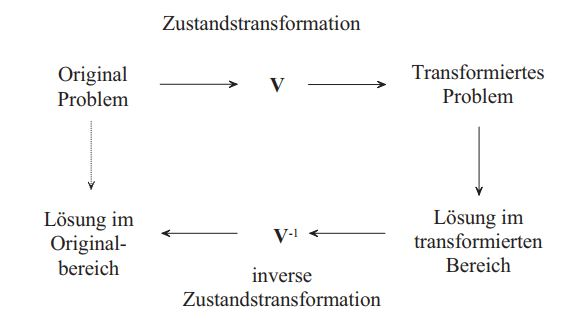
\includegraphics[width=0.4\linewidth]{./pics/re/zsttrans}
				\caption{Reguläre Zustandstransformation}
			\end{figure}
			\leavevmode \\
			Auch wird die Matrix $ \tilde{\bm{A}}= \bm{V}^{-1}\bm{AV}$ gerne in eine Begleitmatrix der Form
			\[ \tilde{\bm{A}} = \begin{bmatrix}0 & 1 & 0 & \dotsm & 0 \\
			0 & 0 & 1 & \dotsm & 0 \\
			\vdots & \vdots & \vdots & \ddots & \vdots\\
			0 & 0 & 0 & \dotsm & 1 \\
			-a_{0} & -a_{1} & -a_{2} & \dotsm & -a_{n-1} \\\end{bmatrix}\]
			umgewandelt, da diese Darstellungen nützlich für den Reglerentwurf sind (als Beispiel sei die Polvorgabe gegeben) oder Systemeigenschaften direkt abgelesen werden können.
			
		\subsubsection{Nichtlineare Zustandstransformation}
			Auch bei nichtlinearen Systemen
			\[\bm{\dot{x}} = \bm{f}(\bm{x,u}) \]
			können Transformationen
			\[\bm{z} = \bm{q}(\bm{x}), \qquad \bm{x} = \bm{q}^{-1}(\bm{z}) \]
			sinnvoll sein, wenn es gelingt, das System in eine für den Reglerentwurf geeignete Form zu bringen. Für die Transformation wird gefordert, dass sie stetig differenzierbar und eindeutig ist. Eindeutig bedeutet, dass jedem $ \bm{x} $ genau ein $ \bm{z} $ zugeordnet ist und umgekehrt. Dadurch ist auch gefordert, dass die Anzahl der Zustände durch eine nichtlineare Zustandstransformation gleich bleibt. Eine solche Transformation nennt man \hyperref[diffeomorphismus]{Diffeomorphismus}. Das transformierte System ergibt sich durch Substitution zu
			\[\dfrac{\partial \bm{q}^{-1}(\bm{z})}{\partial \bm{t}}  = \bm{f}(\bm{q}^{-1}(\bm{z}),\bm{u}) 
			\qquad \Rightarrow \qquad
			\dfrac{\partial \bm{q}^{-1}(\bm{z})}{\partial \bm{z}} \dot{\bm{z}} = \bm{f}(\bm{q}^{-1}(\bm{z}),\bm{u}),  \] 
			woraus sich die transformierte Systemdarstellung 
			\[\Rightarrow \qquad 
			 \dot{\bm{z}} = \bigg(\dfrac{\partial \bm{q}^{-1}(\bm{z})}{\partial \bm{z}}\bigg)^{-1}\cdot \bm{f}(\bm{q}^{-1}(\bm{z}),\bm{u}) = \tilde{\bm{f}}(\bm{z,u}) \]
			 ergibt. Da die Transformation eindeutig ist, gibt es auch eine Rücktransformation
			 \[ \dot{\bm{x}} = \bigg(\dfrac{\partial \bm{q}(\bm{x})}{\partial \bm{x}}\bigg)^{-1}\cdot \bm{\tilde{f}}(\bm{q}(\bm{x}),\bm{u}) = \bm{f}(\bm{x,u}). \]
			 Im allgemeinen kann es sein, dass die Transformationsgleichung auch eine Abhängigkeit vom Eingangsvektor $ \bm{u} $ und eventuell seinen zeitlichen Ableitungen aufweist. D.h. die Form
			 \[\bm{z} = \bm{q}(\bm{x,u,\dot{u}, ...,u}^{(i)}) \]
			 \[\bm{x} = \bm{q}^{-1}(\bm{z,u,\dot{u}, ...,u}^{(i)}) \]
			 hat. Transformiert man nun das System $ \bm{\dot{x}} = \bm{f}(\bm{x,u}) $ in z-Koordinaten, erhält man
			 \[\dot{x} = \dfrac{\partial \bm{q}^{-1}(\bm{z,u,\dot{u}, ...,u}^{(i)})}{\partial t}= 
			 \dfrac{\partial \bm{q}^{-1}(\bm{z,u,\dot{u}, ...,u}^{(i)})}{\partial z}\dot{z} +\sum_{j=0}^{i}\dfrac{\partial \bm{q}^{-1}(\bm{z,u,\dot{u}, ...,u}^{(i)})}{\partial \bm{u}^{(j)}}\bm{u}^{(j+1)}=
			 \bm{f}(\bm{q}^{-1}(\bm{z,u,\dot{u}, ...,u}^{(i)}),\bm{u}) \]
			 und schließlich die transformierte Systembeschreibung
			 \[\Rightarrow \bm{\dot{z}} = 
			 \bigg(\dfrac{\partial \bm{q}^{-1}(\bm{z,u,\dot{u}, ...,u}^{(i)})}{\partial z}\bigg)^{-1}\cdot \bigg(\bm{f}(\bm{q}^{-1}(\bm{z,u,\dot{u}, ...,u}^{(i)}),\bm{u}) -  \sum_{j=0}^{i}\dfrac{\partial \bm{q}^{-1}(\bm{z,u,\dot{u}, ...,u}^{(i)})}{\partial \bm{u}^{(j)}}\bm{u}^{(j+1)}\bigg). \]
			 Mit dem Hintergedanken dass die Zustände $ \bm{x} $ bzw. $ \bm{z} $ auch vom Eingang und seinen Ableitungen abhängt, kann die transformierte folgendermaßen dargestellt werden.
			 \[\Rightarrow \bm{\dot{z}} = 
			 \bigg(\dfrac{\partial \bm{q}^{-1}}{\partial z}\bigg)^{-1}\cdot \bigg(\bm{f}(\bm{q}^{-1},\bm{u}) -  \sum_{j=0}^{i}\dfrac{\partial \bm{q}^{-1}}{\partial \bm{u}^{(j)}}\bm{u}^{(j+1)}\bigg) = \tilde{\bm{f}}(\bm{z,u})\]
			 
			 \textsc{Nichtlineare Systeme und Regelungen, Jürgen Adamy S207}
			 \paragraph{Herleitung des Diffeomorphismus (Transformationsvorschrift \textit{ q})}
			 TODO				
			
	\subsection{Eingangstransformation}
		
\section{Stabilität}
	\subsection{Stabilitätsanalyse des charakteristischen Polynoms}	
		Bei linearen Systemen ist das Nennerpolynom der Übertragungsfunktion das charakteristische Polynom, wobei dessen Koeffizienten die Nullstellen des Polynoms und somit die Pole des Systems darstellen. Gegeben sei die Differentialgleichung
		\[\dot{y}(t) + a_{0}y(t) = 0. \]
		Mit dem eulerschen Ansatz $ y=e^{\lambda t} $ ergibt sich
		\[e^{\lambda t}(\lambda + a_{0}) = 0\]
		mit dem charakteristischen Polynom $ \lambda + a_{0} = 0 $. Dieses Polynom hat die Nullstelle 
		\[\lambda=-a_{0}.\]
		In den Ansatz eingesetzt ergibt sich
		\[ y(t)=e^{-a_{0} t}. \]
		Dadurch ergibt sich für unendliche Zeit und einem negativen Realteil von $ a_{0} $
		\[\lim\limits_{t\mapsto \infty}(e^{-a_{0} t}) = 0.\]
		Die Differentialgleichung heißt dann asymptotisch stabil. Für Differentialgleichungen höherer Ordnungen werden etwa das \textit{Hurwitz}- oder \textit{Routh}-Kriterium verwendet um die stabilität von DGL's zu prüfen.
	
\section{Eigenschaften eines Regelkreises}
	\subsection{Bandbreite}
		Die Bandbreite eines Regelkreises ist jene Frequenz, bei der der Amplitudenverlauf des Bode Diagramms, die -3dB Grenze unterschreitet. Höhere Bandbreite bedeutet, dass der Regelkreis (das geregelte System) seinem Sollwert bis zu höheren Frequenzen folgen kann.
		\begin{figure}[h]
			\centering
			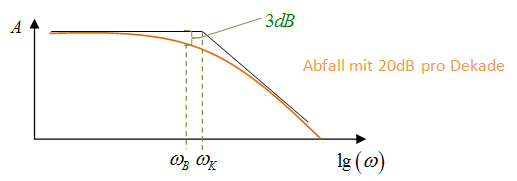
\includegraphics[width=0.7\linewidth]{./pics/re/band}
			\caption{Amplitudenverlauf: $ \omega_{B} $ - Bandbreite des Systems, $ \omega_{K} $ - Knickfrequenz}
			\label{}
		\end{figure}
		\leavevmode \\
	
	\subsection{\textcolor{red}{Nyquist-Diagramm}}
	\subsection{\textcolor{red}{Wurzelortskurve}}
	\subsection{\textcolor{red}{Empirische Grundformeln}}
	\subsection{Führungs- und Störungsverhalten eines Regelkreises}


\section{Identifikation von Systemen}

\section{Systemdarstellung: Normal- und Regelungsformen}
	\subsection{Normalformen}
	\subsubsection{Regelungsnormalform \textit{(auch Steuerungsnormalform)}}
	\subsubsection{Beobachtungsnormalform}
	\subsubsection{Kanonische Normalform}
	\subsubsection{Brunovsky–Normalform}
	\subsubsection{Jordansche-Normalform}
	\subsubsection{Nichtlineare Regelungsnormalform} \label{chapNL}
		Nichtlineare eingangsaffine Systeme der Form
		\begin{equation}
			\dot{\bm{x}}=\bm{a(x) + B(x)}\cdot u =\bm{a(x)}+\sum_{i=1}^{m}\bm{b}_{i}(u)\cdot u_{i}
			\label{nlrnf}
		\end{equation}

		können in der nichtlinearen Regelungsnormalform
		\[\begin{bmatrix}\dot{x}_{1}\\\vdots\\ \dot{x}_{n-1}\\\dot{x}_{n}\end{bmatrix} =
		\begin{bmatrix}x_{2}\\\vdots\\ x_{n}\\\alpha(\bm{x})\end{bmatrix} + 
		\begin{bmatrix}0\\\vdots\\ 0\\\beta(\bm{x})\end{bmatrix}u\]
		\[y = x_{1}\]	
		dargestellt werden.
		\begin{figure}[h]
			\centering
			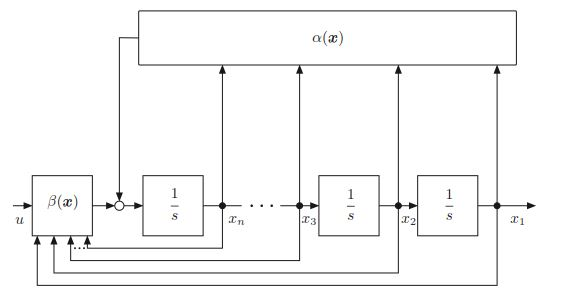
\includegraphics[width=0.6\linewidth]{./pics/re/nlrnf}
			\caption{System in nichtlinearer Regelungsnormalform}
			\label{}
		\end{figure}
		\paragraph{Zustandskoordinatentransformation mittels Lie-Ableitungen}
			Im folgenden wird beschrieben, wie Systeme der Form (\ref{nlrnf}) in die nichtlineare Regelungsnormalform transformiert werden können.\\
			\begin{tcolorbox}[title=Definition: \textit{Lie-Derivierte/Lie-Ableitung}]
				Sie sind als Gradient einer skalaren Funktion $ h(\bm{x}) $ multipliziert mit einem Vektorfeld $ \bm{f(x)} $ definiert
				\[\bm{L_{f}}h(\bm{x}) = \dfrac{\partial h(\bm{x})}{\partial\bm{x}}\bm{f(x)}=grad^{T}h(\bm{x})\cdot \bm{f(x)} \]	
				Die skalare Funktion kann beispielsweise die Ausgangsfunktion $ c(\bm{x}) $ sein und das Vektorfeld z.b. der Dynamikvektor $ \bm{a}(\bm{x}) $.
			\end{tcolorbox}
			Man bildet nun die zeitliche Ableitung der Ausgangsgröße $ y $ und erhält
			\[\dot{y}=\dfrac{dc(\bm{x(t)})}{dt} = \dfrac{\partial c(\bm{x})}{\partial x_{1}}\underbrace{\dfrac{\partial x_{1}(t)}{\partial t}}_{\dot{x}_{1}} + ... + \dfrac{\partial c(\bm{x})}{\partial x_{n}}\dot{x}_{n} = \dfrac{\partial c(\bm{x})}{\partial \bm{x}}\dot{\bm{x}}.\]
			Durch einsetzen von $ \dot{\bm{x}}=\bm{a(x) + b(x)}\cdot u $ in obige Gleichung, ergibt sich  
			\[\dot{y}=\dfrac{\partial c(\bm{x})}{\partial \bm{x}}\bm{a(x)} + \dfrac{\partial c(\bm{x})}{\partial \bm{x}}\bm{b(x)}\cdot u. \]
			Geschrieben mit den Lie-Derivierten:
			\[\dot{y}=L_{\bm{a}}c(\bm{x})+ L_{\bm{b}}c(\bm{x})\cdot u \]
			Für die meisten technischen Systeme ist der zweite Term gleich Null, woraus 
			\[\dot{y}=L_{\bm{a}}c(\bm{x})\]
			folgt.
			Die zweite Ableitung ergibt sich dann zu
			\[\ddot{y}= \dfrac{dL_{\bm{a}}c(\bm{x})}{dt}= \dfrac{\partial L_{\bm{a}}c(\bm{x})}{\partial \bm{x}}\dot{\bm{x}} = \underbrace{\dfrac{\partial L_{\bm{a}}c(\bm{x})}{\partial \bm{x}}\bm{a(x)}}_{L_{\bm{a}}L_{\bm{a}}c(\bm{x})}+\underbrace{\dfrac{\partial L_{\bm{a}}c(\bm{x})}{\partial \bm{x}}\bm{b(x)}}_{L_{\bm{b}}L_{\bm{a}}c(\bm{x})}\cdot u = L_{\bm{a}}L_{\bm{a}}c(\bm{x}) + L_{\bm{b}}L_{\bm{a}}c(\bm{x})\cdot u.\]
			Mit dem zweiten Term wieder zu Null folgt
			\[\ddot{y}=L_{\bm{a}}L_{\bm{a}}c(\bm{x}) = L_{\bm{a}}^{2}c(\bm{x})\]
			Bildet man auch die höheren Ableitungen, so ergibt sich schließlich folgendes Ergebnis:
			\begin{eqnarray} 
				y &=& c(\bm{x})\nonumber\\
				\dot{y}&=&L_{\bm{a}}c(\bm{x})\nonumber\\
				\ddot{y}&=&L_{\bm{a}}^{2}c(\bm{x})\nonumber\\
				\vdots \nonumber\\
				y^{(\delta-1)} &=&L_{\bm{a}}^{(\delta-1)}c(\bm{x})   \nonumber\\
				y^{(\delta)} &=&L_{\bm{a}}^{(\delta)}c(\bm{x}) + L_{\bm{b}}L_{\bm{a}}^{(\delta-1)}c(\bm{x})\cdot u   \nonumber\\
			\end{eqnarray}
			Leitet man die Ausgangsfunktion $ \delta- $mal, so dass die Stellgröße $ u $ darin auftaucht, nennt man $ \delta $ den relativen Grad des Systems. Es wird nun lediglich der Fall
			\[\delta = n\]
			betrachtet, also der Fall bei dem der relative Grad gleich der Systemordnung entspricht.
			Weiter führen wir die neuen Zustandskoordinaten $ \bm{z} $ ein.
			\[\bm{z}=\begin{bmatrix}z_{1}\\z_{2}\\z_{3}\\\vdots\\ z_{n}\end{bmatrix} = 
			\begin{bmatrix}y\\\dot{y}\\\ddot{y}\\\vdots\\ y^{(n-1)}\end{bmatrix} =
			\begin{bmatrix}c(\bm{x})\\L_{\bm{a}}c(\bm{x})\\L_{\bm{a}}^{2}c(\bm{x})\\\vdots\\ L_{\bm{a}}^{(n-1)}c(\bm{x})\end{bmatrix} = \bm{t}(\bm{x})\]
			Ist $ \bm{t}(\bm{x}) $ stetig differenzierbar und es existiert die Umkehrfunktion 
			\[\bm{t}^{-1}(\bm{t}(\bm{x}))=\bm{x},\]
			dann nennt man $ \bm{t} $ einen \textit{Diffeomorphismus}. Durch Differenziation der Transformationsgleichung $ bm{t}(\bm{x}) $ erhalten wir die nichtlineare Regelungsnormalform.
			\[\bm{\dot{z}}=\begin{bmatrix}\dot{z}_{1}\\\dot{z}_{2}\\\dot{z}_{3}\\\vdots\\ \dot{z}_{n}\end{bmatrix} = \begin{bmatrix}\dot{y}\\\ddot{y}\\\dddot{y}\\\vdots\\ y^{(n)}\end{bmatrix} = \begin{bmatrix}z_{2}\\z_{3}\\z_{4}\\\vdots\\ z_{n+1}\end{bmatrix} =\bm{\dot{t}}(\bm{x}) = \begin{bmatrix}L_{\bm{a}}c(\bm{x})\\L_{\bm{a}}^{2}c(\bm{x})\\\vdots\\ L_{\bm{a}}^{(n-1)}c(\bm{x})\\ L_{\bm{a}}^{(n)}c(\bm{x}) + L_{\bm{b}}L_{\bm{a}}^{(n-1)}c(\bm{x})\cdot u\end{bmatrix}\]
			\[\Rightarrow\begin{bmatrix}\dot{z}_{1}\\\vdots\\\dot{z}_{n-1}\\ \dot{z}_{n}\end{bmatrix} = \begin{bmatrix}z_{2}\\\vdots\\ z_{n}\\\alpha(\bm{x})\end{bmatrix}+\begin{bmatrix}0\\\vdots\\ 0\\\beta(\bm{x})\end{bmatrix}u,\]
			mit
			\begin{eqnarray} 
			\alpha(\bm{x}) &=& L_{\bm{a}}^{(n)}c(\bm{x}) \nonumber\\
			\beta(\bm{x}) &=& L_{\bm{b}}L_{\bm{a}}^{(n-1)}c(\bm{x}) \nonumber
			\end{eqnarray}
			
	\subsubsection{Byrnes-Isidori-Normalform}
	
	
\section{Arten von Regelstrecken}
	\begin{itemize}
		\item  linear, nichtlinear
		\item statisch, dynamische
		\item zeitvariant, zeitinvariant
		\item SISO, MIMO
	\end{itemize}

\section{Arten von Reglern}
	\begin{itemize}
		\item Realisierung als Analoger- und digitaler Regler
		\item Stetige lineare Regler
		\begin{itemize}
			\item PID-Regler
			\item Zustandsregler
		\end{itemize}
		\item Unstetige Regler
		\begin{itemize}
			\item Zweipunktregler
			\item Dreipunktregler
			\item Mehrpunktregler
		\end{itemize}
		\item Nichtlineare Regler
		\begin{itemize}
			\item Adaptiver Regler
			\item Fuzzy-Regler
		\end{itemize}
	\end{itemize}
	\subsection{Standardregelkreis}
		Der Standardregelkreis ist ein Regelkreis mit Ausgangsrückführung. Dabei wird lediglich das Eingangs-/Ausgangsverhalten des Systems betrachtet. Die Regelstrecke kann auch als Zustandsraummodell mit Zustandsvariablen beschreiben werden, jedoch wird
		\begin{figure}[h]
			\centering
			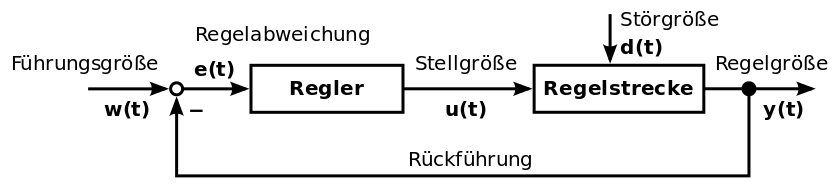
\includegraphics[width=0.7\linewidth]{./pics/re/std}
			\caption{Standardregelkreis mit Ausgangsrückführung}
		\end{figure}
		Regler können anhand von Frequenzlinienverfahren oder durch vorgeben der Zähler- und Nennerpolynome der Übertragungsfunktion (Polvorgabe) entworfen werden. Bei vorhandener Übertragungsfunktion kann mittels inverser Laplace-Transformation der zeitliche Verlauf der Ausgangsgröße errechnet und durch die Parameterwahl vorgegeben werden. 
	\subsection{Zustandsregler}
		Der \textit{Standardregelkreis} und dazugehörige Frequenzkennlinienverfahren beruhen auf einer Regelkreisstruktur, bei der eine Größe, die so genannte Ausgangsgröße, gemessen wird, und auf deren Kenntnis gemeinsam mit der vorgegebenen Führungsgröße der Regler als dynamisches System die Stellgröße errechnet. Daher werden Regelkreise dieser Art auch als Ausgangsregelungen bezeichnet. Setzt man nun voraus, dass der gesamte Zustand eines Systems messtechnisch erfassbar ist, dann ist es möglich, einen so genannten \textit{Zustandsregler} zu entwerfen. Die Zustandsvariablen eines Systems sind frühzeitiger als der Ausgang vorhanden, was zu einer schnellen Regelung führt.
		\begin{figure}[h]
			\centering
			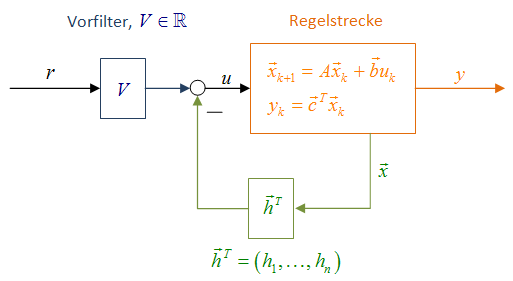
\includegraphics[width=0.7\linewidth]{./pics/re/zust}
			\caption{Zustandsregler mit $ h^{T} $ zur Vorgabe der Systemdynamik und $ V $ zur Elimination des statischen Fehlers}
		\end{figure}
		\leavevmode\\
		Durch die Hintereinanderschaltung der Integratoren ist nur die Zustandsvariable x1(t) = y(t) eine stationäre Größe, wenn die Eingangsgröße 	$ 	u ( t )$ konstant ist. Alle anderen Zustandsvariablen – eine stabile Regelstrecke vorausgesetzt – streben gegen den Wert null. Nach Einstellung und Optimierung des Faktors k1 ergibt sich ein stabiler Regelkreis bestimmter Dämpfung mit einem Proportionalfehler der Regelgröße	$ y ( t ) $	gegenüber 
		$ 	w ( t ) $. Die anderen Faktoren der Zustandsvariablen werden hintereinander beispielsweise zur Optimierung des Übergangsverhaltens eingestellt.
		Ein Vorfilter vor dem Soll-Ist-Vergleich korrigiert den statischen Fehler zwischen $ 	w ( t ) $ und 	$ 	y ( t ) $. Durch Einfügen eines überlagerten PI-Reglers verschwinden die Nachteile des einfachen Zustandsreglers. Das Vorfilter wird dann nicht mehr benötigt.\\\\
		Durch die Zustandsrückführung kann keine stationäre Genauigkeit der Regelgröße zum Sollwert erreicht werden. Selbst bei einer Regelstrecke ohne Nullstellen, also ohne differenzielle Anteile, ist die Zustandsvariable $ x_{1} $ nach der Regelungsnormalform nicht identisch mit der Ausgangsgröße $ y(t) $. Deshalb wird die Zustandsrückführung häufig mit einem Vorfilter $ V $ erweitert. Die Führungsgröße $ w ( t ) $ wirkt direkt auf das Vorfilter. Für einfache Anforderungen kann mittels eines Faktors in dem Vorfilter eine Korrektur durchgeführt werden, damit im stationären Zustand $ 	w ( t ) = y ( t ) $ erreicht wird.

\section{Auslegung von Reglern}
	\subsection{Reglerauslegung durch Polvorgabe}
	\subsection{Frequenzkennlinienverfahren}

\section{Arten von Rückführungen}
	\subsection{Ausgangsrückführung}
		Die klassische Ausgangsrückführung $ \bm{u}=\bm{K(w-y)} $ stand am Anfang der Entwicklung der Regelungstechnik. Diese Art der Rückführung wird meist im \textsc{laplace}-Bildbereich untersucht und es spielt dabei nur das Eingangs-/Ausgangsverhalten eine Rolle.
	\subsection{Zustandsrückführung}
		Für komplexere Regelungsaufgaben kommen Zustandsrückführungen zum Einsatz.
		\[\bm{u}=\bm{R_{u1}x}+\bm{R_{u2}v}\]
		Sie ist die allgemeinere Rückführungsart der Beiden und umfasst somit auch die Ausgangsrückführung. Betrachtungen von Zustandsmodellen finden meist im Zeitbereich statt. Hauptanwendungen sind \textit{exakte Linearisierungen} oder \textit{Entkoppelungen} die das System in mehrere Teilsysteme aufteilt, die dann unabhängig voneinander gesteuert oder geregelt werden können.
		\subsubsection{Statische Zustandsrückführung}
			Bei der statischen Zustandsrückführung ist charakteristisch, dass die Eingangsgröße $ \bm{u} $ von den Zustandsgrößen und der neuen Eingangsgröße $ \bm{v} $ abhängig ist.
			\[\bm{u}=\bm{r(x)}+\bm{R(x)v}\]
			\begin{figure}[h]
				\centering
				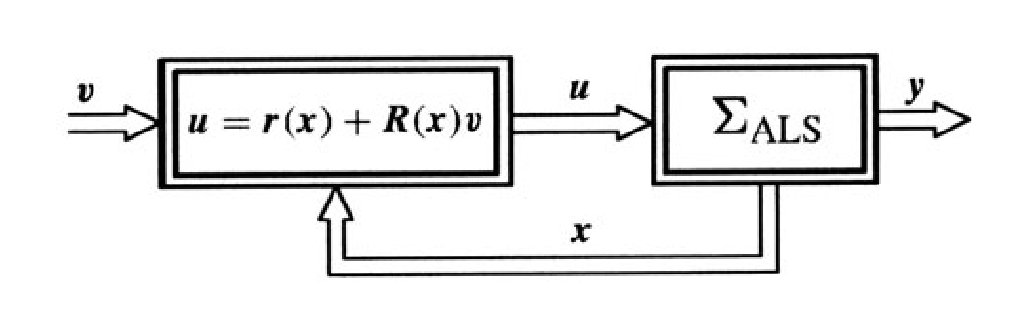
\includegraphics[width=0.6\linewidth]{./pics/re/stat}
				\caption{Statische Zustandsrückführung; $ \Sigma_{ALS} $ bedeutet \textit{analytisches Modell mit linear eingehender Steuerung}}
			\end{figure}
		\subsubsection{Quasi-statische Zustandsrückführung}
			Bei der quasi-statischen Rückführung ist $ \bm{u} $ zusätzlich von den Ableitungen des neuen Eingangs $ \bm{v} $ abhängig. Jedoch wird der Zustandsvektor nicht wie bei der dynamischen Rückführung erweitert, sondern behält seine Dimension.
		\subsubsection{Dynamische Zustandsrückführung}
			Bei der dynamischen Rückführung treten zusätzliche Differentialgleichungen in einer neuen internen Variable $ z $ auf. Ist die neue Eingangsgröße $ \bm{v} $ linear, ergibt sich die Stellgröße zu
			\[\bm{\dot{z}}=\bm{r}_{z}(\bm{x,z})+\bm{R}_{z}(\bm{x,z})\bm{v}\]
			\[\bm{u} = \bm{r}_{u}(\bm{x,z})+\bm{R}_{u}(\bm{x,z})\bm{v}\]
			\begin{figure}[h]
				\centering
				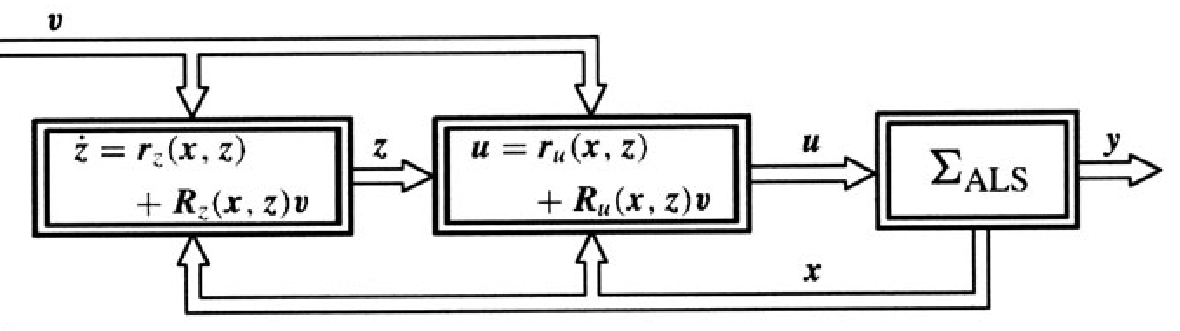
\includegraphics[width=0.7\linewidth]{./pics/re/dyn}
				\caption{Dynamische Zustandsrückführung}
			\end{figure}


\section{Stellgrößenbeschränkung}
	\subsection{Anti-Windup Maßnahmen bei Reglern mit I-Anteil}
		
\section{Regelungen für nichtlineare Strecken}
	\subsection{Linearisungsmethoden}
		\subsubsection{Taylor-Linearisierung}
		\subsubsection{Carleman-Linearisierung}
		\subsubsection{Feedback-Linearisierung}
		\subsubsection{Harmonische-Linearisierung}
	\subsection{Reglerentwurf mittels exakter Eingangs-/Ausgangslinearisierung}
		\subsubsection{Bei maximalem relativen Grad $ \delta=n $ von SISO-Systemen}
			Grundidee ist es direkt und nicht über den Umweg einer linearen Näherung (wie vorherige Kapitel) einen Regler für das nichtlineare System zu entwerfen. Grundgedanke hierbei ist einen nichtlinearen Regler auszulegen der das nichtlineare Verhalten der Strecke kompensiert und so insgesamt ein linearer Regelkreis entsteht. Die exakte Linearisierung wird auch Eingangs-/Ausgangslinearisierung genannt und linearisiert demnach das Verhalten zwischen Eingangs- und Ausgangsgröße. Die interne Dynamik bleibt dabei nichtlinear.  Voraussetzung ist ein eingangsaffines nichtlineares System das in nichtlinearer Regelungsnormalform vorliegt oder in eine solche überführt werden kann.
			\[\bm{\dot{x}} = \bm{a(x)} + \bm{b(x)}u \]
			\[y=c(\bm{x})\]
			In der \textit{nichtlinearen Regelungsnormalform} 
		 	\[\Rightarrow\begin{bmatrix}\dot{z}_{1}\\\vdots\\\dot{z}_{n-1}\\ \dot{z}_{n}\end{bmatrix} = \begin{bmatrix}z_{2}\\\vdots\\ z_{n}\\\alpha(\bm{x})\end{bmatrix}+\begin{bmatrix}0\\\vdots\\ 0\\\beta(\bm{x})\end{bmatrix}u,\]
		 	\[y = z_{1}\]	
			Mit dem System in nichtlinearer Regelungsnormalform, erhält man mit dem Regelgesetz
			\[u = - \dfrac{\alpha(\bm{x})+\sum_{i=1}^{n}a_{i-1}\cdot z_{i}}{\beta(\bm{x})} + \dfrac{V}{\beta(\bm{x})}w\]
			den linearen geschlossenen Regelkreis in Regelungsnormalform
			\[\begin{bmatrix}\dot{z}_{1}\\\dot{z}_{2}\\\vdots\\\dot{z}_{n-1}\\ \dot{z}_{n}\end{bmatrix} = \begin{bmatrix}0 & 1 & 0 & \dotsm & 0 \\
			0 & 0 & 1 & \dotsm & 0 \\
			\vdots & \vdots & \vdots & \ddots & \vdots\\
			0 & 0 & 0 & \dotsm & 1 \\
			-a_{0} & -a_{1} & -a_{2} & \dotsm & -a_{n-1} \\\end{bmatrix}
			\begin{bmatrix}z_{1}\\z_{2}\\\vdots\\z_{n-1}\\ z_{n}\end{bmatrix}+	\begin{bmatrix} 0\\0\\\vdots\\0\\V\end{bmatrix}w,\]
			für den das Verhalten wie gewohnt durch Polvorgabe gewählt werden kann.\\\\			
			\textbf{Erweiterung auf allgemeinere Systeme:\\}
			Für den gezeigten Fall muss das System in nichtlinearer Regelungsnormalform vorliegen. Da dies nicht oft so ist, muss eine Zustandskoordinatentransformation durchgeführt werden, die das System in die nichtlineare Regelungsnormalform transformiert. Für diesen Zweck werden die \textit{Lie-Derivierte} oder \textit{Lie-Ableitungen} verwendet. (Siehe Kapitel \ref{chapNL})
			\begin{figure}[h]
				\centering
				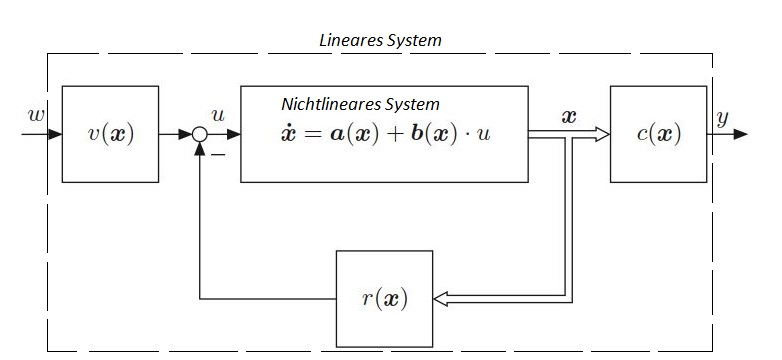
\includegraphics[width=0.8\linewidth]{./pics/re/dlin}
				\caption{Strukturbild des Regelkreises mit insgesamt linearer Dynamik}
			\end{figure}
			\leavevmode\\
			Man nennt die beschriebene Vorgehensweise \underline{\textbf{exakte Linearisierung bei maximalem relativen Grad.}} Mit exakter Linearisierung ist hierbei genau genommen die \textit{exakte Eingangs-/Ausgangslinearisierung} gemeint.\\\\
			Für die Differentialgleichung der Ausgangsgröße $ y $ ergibt sich folgendes lineares Verhalten aus obigem Zustandsraummodell:
			\[y^{(n)}+a_{n-1}y^{(n-1)} + ... + a_{1}\dot{y}+a_{0}y=V\cdot w.\]
			Setzt man in obiges Regelgesetz $ \alpha $ und $ \beta $ ein und ersetzt $ \bm{z} $ mit
			\[\bm{z}=\bm{t}(\bm{x})=\begin{bmatrix}c(\bm{x})\\L_{\bm{a}}c(\bm{x})\\L_{\bm{a}}^{2}c(\bm{x})\\\vdots\\ L_{\bm{a}}^{(n-1)}c(\bm{x})\end{bmatrix},\]
			erhält man die \textit{nichtlineare Ackermann-Formel}\\
			\begin{tcolorbox}[title=Definition: \textit{nichtlineare Ackermann-Formel}]
				\[u=-\dfrac{L_{\bm{a}}^{(n)}c(\bm{x})+a_{n-1}L_{\bm{a}}^{(n-1)}c(\bm{x})+...+a_{1}L_{\bm{a}}c(\bm{x})+a_{0}c(\bm{x})}{L_{\bm{b}}L_{\bm{a}}^{(n-1)}c(\bm{x})}+\dfrac{V}{L_{\bm{b}}L_{\bm{a}}^{(n-1)}c(\bm{x})}w\]
				[\textsc{Nichtlineare Systeme und Regelungen, Jürgen Adamy S292}]
			\end{tcolorbox}
		
		
		\subsubsection{Bei reduziertem relativen Grad $ \delta<n $ von SISO-Systemen}	
			Ist der relative Grad $ \delta < n $, dann bleibt eine nichtlineare interne Dynamik übrig. Die Zustandsvariablen der internen Dynamik verhalten sich nichtlinear, wirken sich jedoch nicht auf die Ausgangsgröße aus. Voraussetzung für die Stabilität des Gesamtsystems ist jedoch auch die Stabilität der internen Dynamik.\\	
	\subsection{Exakte Zustandslinearisierung}
		Auch \textbf{exakte Eingangs-Zustandslinearisierung} genannt.\\\\
		Bei der exakten Eingangs-/Ausgangslinearisierung ist das System exakt linearisierbar, wenn $ \delta=n $ gilt. Ist der relative Grad jedoch kleiner als die Systemordnung, dann kann die Linearisierung nicht für alle Zustände durchgeführt werden. Es bleibt somit eine nichtlineare interne Dynamik. Bei der exakten Zustandslinearisierung wird ein \textit{fiktiver} Ausgang $ y $ gesucht für den wieder $ \delta=n $ gilt und die exakte Linearisierung somit durchführbar ist.\\\\
		Systeme ohne Ausgang??\\\\
		Brunovsky-Normalform [\textsc{Nichtlineare Systeme und Regelungen, Jürgen Adamy S337}]
		
	\subsection{Nonlinear Model predictive control (NMPC)}
		Auf Basis eines zeitdiskreten dynamischen Systems wird der zukünftige Verlauf vorhergesagt. Dieser ist abhängig von den Eingangssignalen, die so gewählt werden, dass sich der vorhergesagte Verlauf, einer gewünschten Kurve annähert. Die Berechnung der optimalen Eingangssignale erfolgt über eine Kostenfunktional. Durch dessen Minimierung erhält man den optimalen Ausgangsverlauf. Die Optimierung wird in jedem Zeitschritt erneut, mit neuen Messdaten durchgeführt $ \rightarrow  $ ressourcenintensiv.
		\begin{figure}[h!]
			\centering
			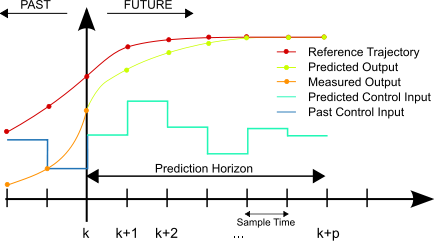
\includegraphics[width=0.5\linewidth]{./pics/re/nmpc}
		\end{figure}\\
		Die nichtlineare Modellprädiktive Regelung bietet eine Möglichkeit für die Prozessmodellierung, wenn diese Prozesse nicht linearisiert werden sollen.\\\\
		\textbf{\underline{Vorteile \& Nachteile}:}
		\begin{itemize}
			\item[+] keine Linearisierung nötig
			\item[-] Zeitintensive Berechnung der Optimierungsfunktion im nichtlinearen Fall. Daher auch nur für langsame Regelstrecken (z.B. Prozessindustrie) einsetzbar.
			\item[-] Optimierung des Kostenfunktionals muss in jedem Schritt durchgeführt werden
		\end{itemize}
	\subsection{Flachheitsbasierter Ansatz}
		Bei der Regelung von Robotern ist man mit der Aufgabe der Folgeregelung bzw. Bahnverfolgung konfrontiert. Der Endeffektor soll eine vorgegebene Bahn abfahren, während	dieses Bewegungsvorgangs ändert sich das Systemverhalten kontinuierlich. Infolge des großen
		Arbeitsbereichs ist die Annahme eines linearisierten Modells nicht ausreichend, deshalb ist eine nichtlineare Modellbildung erforderlich. Für nichtlineare Modelle, die als flach charakterisiert	werden können, vereinfacht sich die Trajektorienregelung wesentlich. Denn bei diesem Verfahren wird durch eine Rückführung die Dynamik des Folgefehlers linearisiert. Der Dynamik des geregelten Systems wird dagegen kein lineares Verhalten aufgeprägt. Daraus resultiert ein geringer Aufwand bei der Auslegung leistungsfähiger Regler, außerdem können eine Vielzahl technischer Anlagen als flache Systeme modelliert werden.\\\\
		Nichtlineare flache Systeme können in geeigneten Koordinaten wie lineare Systeme in linearen Räumen dargestellt werden.  Die neuen Koordinaten stehen mit den Originalkoordinaten in einem (formal eindeutig umkehrbaren) nichtlinearen Zusammenhang. Die so eingeführten nichtlinearen
		Koordinatentransformationen können als dynamische Rückführungen interpretiert werden. \\\\	
		Der flachheitsbasierte Entwurf einer nichtlinearen Folgeregelung geschieht in zwei Stufen: Zunächst erfolgt eine Planung der Trajektorie zur Beschreibung des Sollverhaltens. Dann wird die Folgebewegung entlang der Solltrajektorie durch eine Regelung stabilisiert.\\\\
		In erster Linie kann durch den flachen Ausgang die Steuerung in einfacher Weise entworfen werden, indem die Eingangsgrößen anhand der Ausgangsgrößen berechnet werden. Die Ausgangsgröße ist der gewünschte Trajektorienverlauf, den man beliebig wählen kann. 
		\[\bm{u} =\bm{\varPsi}_{2}(\bm{y,\dot{y},...,y}^{(\beta+1)}) \]
		\begin{figure}[h]
			\centering
			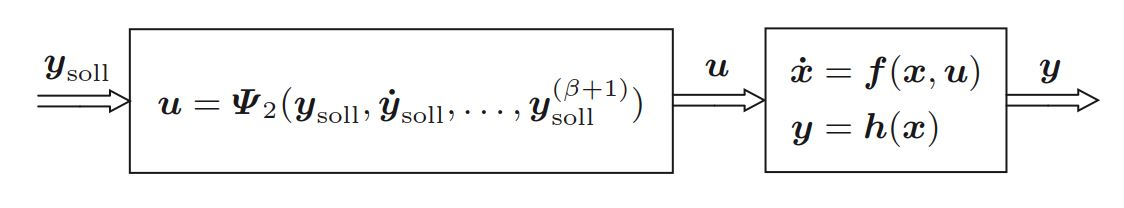
\includegraphics[width=0.6\linewidth]{./pics/re/steuerung}
			\caption{Steuerung eines flachen Systems}
			\label{}
		\end{figure}
		Bei Einwirkung von Störgrößen weicht $ \bm{y}$ vom gewünschten Verlauf $ \bm{y}_{soll} $ ab. Daher ist eine Regelung Strecke nötig um den vorgegebenen Verlauf zu ermöglichen.
		\begin{figure}[h]
			\centering
			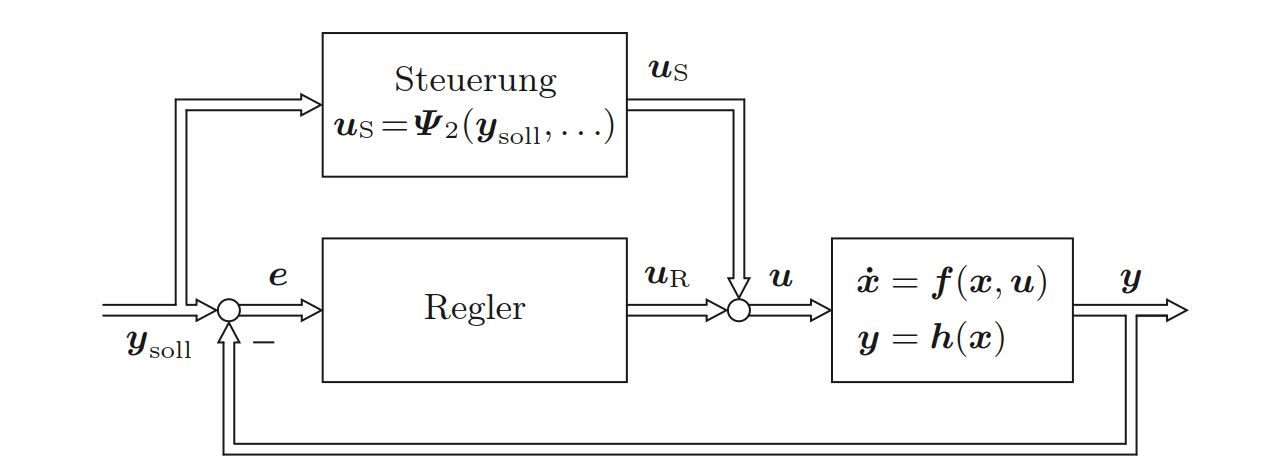
\includegraphics[width=0.6\linewidth]{./pics/re/flach}
			\caption{Flachheitsbasierte Steuerung und Regelung eines flachen Systems}
			\label{}
		\end{figure}
		\leavevmode \\
	\subsection{Gain-scheduling-Regler}
		Ein nichtlineares System der Form \textit{(d ... einwirkende Störgröße)}
		\[\bm{\dot{x}} = \bm{f}(\bm{x},\bm{u},\bm{d}) \]
		kann in einem Arbeitspunkt linearisiert werden und für das linearisierte System kann dann ein Regler entworfen werden der das System lokal stabilisiert. Je weiter man sich jedoch von diesem Arbeitspunkt wegbewegt, desto schlechter funktioniert der Regler.\\
		Wird ein nichtlineares System nicht nur um einen Arbeitspunkt betrieben, ist es sinnvoll Regler zu entwerfen die nicht nur lokale Gültigkeit haben.\\
		Beim \textit{Gain-sheduling-Regler} werden mehrere Arbeitspunkte des Systems linearisiert (parametrierte Linearisierungsfamilie) und für jeden Arbeitspunkt wird mittels linearer Entwurfsmethoden ein entsprechender Regler entworfen. Dafür kommen verschiedene Reglertypen in Frage, z.B. lineare Zustandsregler, PID-Regler, usw.
		\begin{figure}[h]
			\centering
			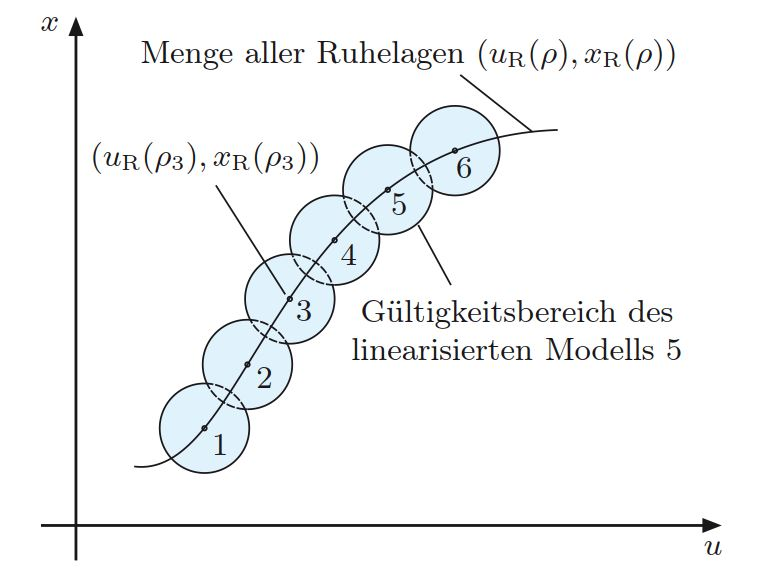
\includegraphics[width=0.5\linewidth]{./pics/re/gain}
			\caption{Gültigkeitsbereiche der parametrierten Linearisierungsfamilie}
		\end{figure}
		\leavevmode \\
		Zwischen den Reglern kann entweder hin und her geschaltet werden, was zu einer abrupten und unerwünschten Änderung der Stellgröße führt oder die Regelparameter werden zwischen den AP'en interpoliert. Die Interpolation kann beispielsweise auf Basis des gewichteten Mittelwertes
		\[\bm{u}=\dfrac{\sum_{i=1}^{p}\mu_{i}\cdot(\overbrace{\bm{u}_{R}(\bm{\rho}_{i})+\Delta\bm{u}_{i})}^{\bm{u}}}{\sum_{i=1}^{p}\mu_{i}}\]
		 erfolgen. Dabei ist $ \mu_{i} $ die Gewichtungsfunktion (z.B. Gauß-Funktion), $ \bm{u}_{R}(\bm{\rho}_{i}) $ die Stellgröße für den \textit{i'ten} Arbeitspunkt und $ \Delta\bm{u}_{i} = \bm{u} - \bm{u}_{R}(\bm{\rho}_{i}) $.
		 \begin{figure}[!h]
		 	\centering
		 	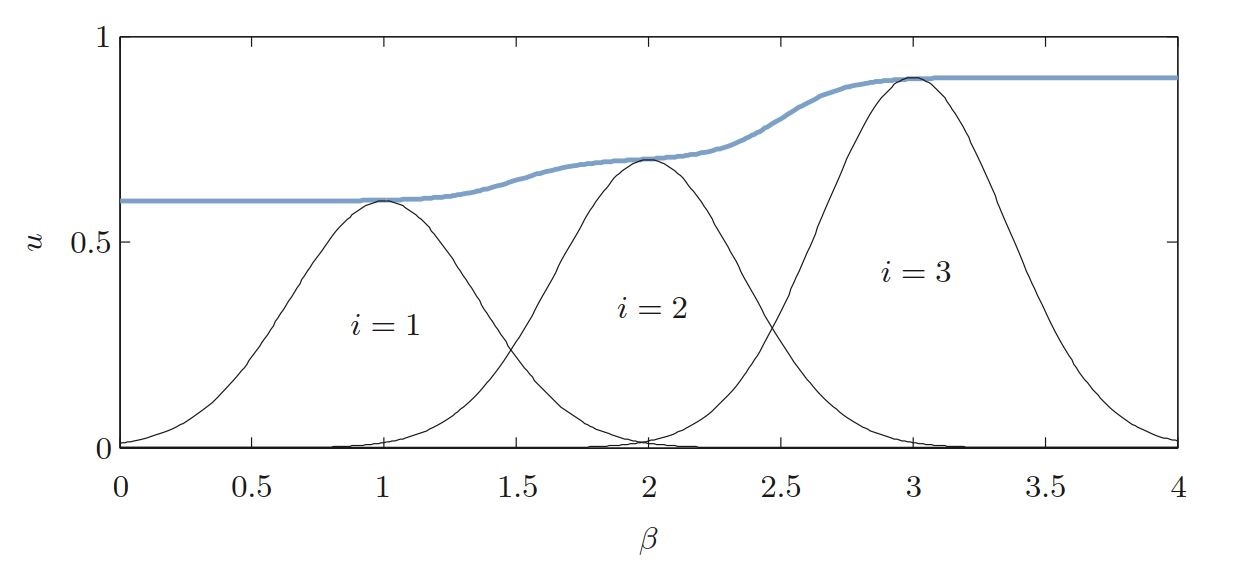
\includegraphics[width=0.8\linewidth]{./pics/re/int}
		 	\caption{Die Interpolation u der Reglerausgangswerte $ \bm{u}_{R}(\bm{\rho}_{i})+\Delta\bm{u}_{i} $ auf Basis des
		 		gewichteten Mittelwertes ist als blaue Kurve exemplarisch dargestellt. Die schwarzen
		 		Kurven entsprechen den Funktionen $\mu_{i}\cdot(\bm{u}_{R}(\bm{\rho}_{i})+\Delta\bm{u}_{i})  $ für i = 1, . . . , 3.}
		 \end{figure}
	 \leavevmode\\\\
	 \textbf{\underline{Zusammenfassung:}}\\\\
	 \textit{Schritt 1:} Berechne parametrierte Linearisierungsfamilie\\
	 \textit{Schritt 2:} Entwerfe die linearen Teilregler mittels linearer Entwurfsmethoden.\\
	 \textit{Schritt 3:} Lege das Auswahl- bzw. Interpolationsgesetz für die Teilregler in Abhängigkeit der Schedulingparameter fest.\\
	 \textit{Schritt 4:} Simuliere den gesamten Regelkreis und prüfe Stabilität und Regelgüte.\\\\
	 \textbf{Man beachte:} Die Stabilität der einzelnen linearen Teilregelkreise reicht nicht aus, da das gesamte System nichtlinear ist. Das heißt, dass die Stabilität im Allgemeinen nicht analytisch gesichert werden kann, sondern simuliert werden muss.\\\\
	 Gain-sheduling Regler: [\textsc{Nichtlineare Systeme und Regelungen, Jürgen Adamy S273}]
	 
		
	\subsection{Control-Ljapunov-Funktionen}
	\subsection{Backstepping-Verfahren}
		Das Backstepping-Verfahren ermöglicht es, Regler und Ljapunov-Funktionen für nichtlineare Regelstrecken in \textit{strenger Rückkopplungsform} zu bestimmen.
		\begin{tcolorbox}[title=Definition: \textit{System vom Typ strenger Rückkopplungsform (engl. strict feedback)}]
			\[\dot{\bm{x}}_{1} = \bm{f}_{1}(\bm{x}_{1})+\bm{h}_{1}(\bm{x}_{1})\cdot x_{2}\]
			\[\dot{x}_{2}= f_{2}(\bm{x}_{1},x_{2})+h_{2}(\bm{x}_{1},x_{2})\cdot x_{3}\]
			\[\vdots\]
			\[\dot{x}_{k}= f_{k}(\bm{x}_{1},x_{2},...,x_{k})+h_{k}(\bm{x}_{1},x_{2},...,x_{k})\cdot u\]
			mit $ \bm{x}_{1}\in \mathbb{R}^{n}$ und $ x_{2},...,x_{k} \in \mathbb{R}.$
		\end{tcolorbox}
	\subsection{Sliding-Mode-Regelung}
		\begin{itemize}
			\item[+] Robustheit gegenüber Regelstreckenparameter-Änderungen, also Änderungen der Dynamikmatrix $ \bm{A} $. Ebenfalls sehr Robust gegenüber von außen einwirkenden Störungen $ \bm{d} $. Genauer wird das Regelgesetz so gewählt, dass die Dynamik des geschlossenen Regelkreises unabhängig von $ \bm{A} $ und $ \bm{d} $ ist.
			\item[-] Durch Schalten des Stellgliedes mit sehr hoher Frequenz während des Gleitens zur Ruhelage folgt ein hoher Verschleiß.
		\end{itemize}
	
	
	
	
	
	
	\newpage
	
		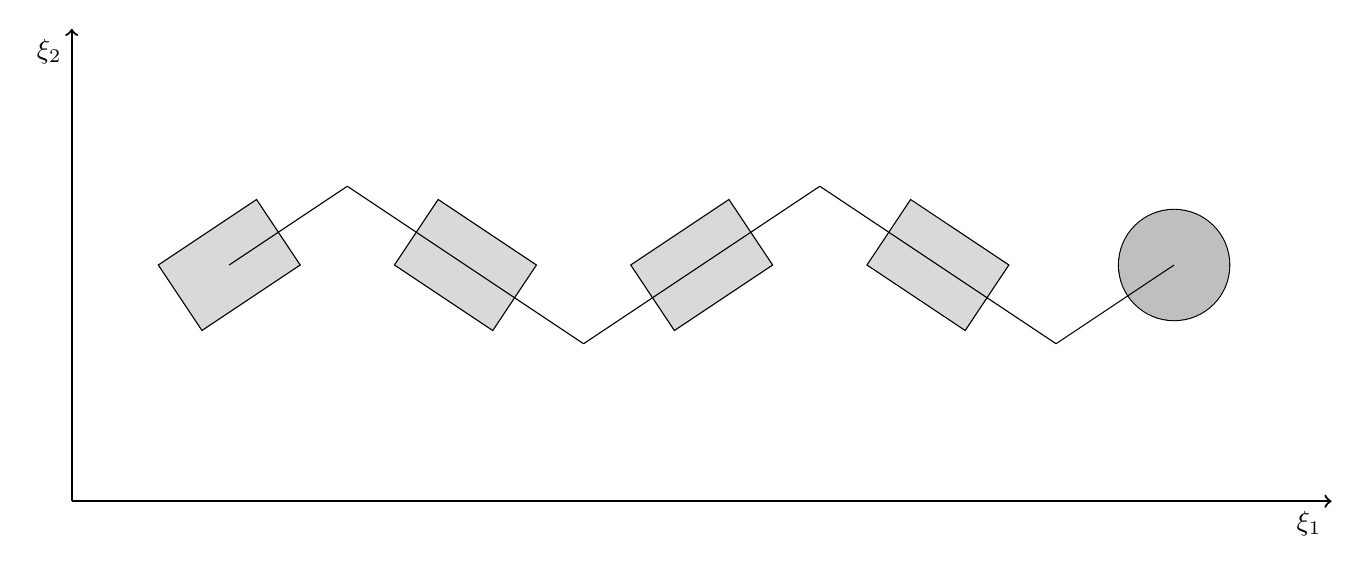
\begin{tikzpicture}
			%[extended line/.style={shorten >=-#1,shorten <=-#1},
			%extended line/.default=1cm,	one end extended/.style={shorten >=-#1}]
			
			% Koordinatensystem
			\draw[thick,->] (0,0) -- (16,0) node[anchor=north east] {$ \xi_{1} $};
			\draw[thick,->] (0,0) -- (0,6)  node[anchor=north east] {$ \xi_{2} $};
			% Fahrzeuge
			\coordinate (x0) at (14,3);
			\coordinate (d0) at (12.5,2);
			\coordinate (x1) at (11,3);
			\coordinate (d1) at (9.5,4);
			\coordinate (x2) at (8,3);
			\coordinate (d2) at (6.5,2);
			\coordinate (x3) at (5,3);
			\coordinate (d3) at (3.5,4);
			\coordinate (x4) at (2,3);
			\pgfmathanglebetweenpoints{\pgfpointanchor{d0}{center}}{\pgfpointanchor{x1}{center}}
			\edef\angP{\pgfmathresult}
			\pgfmathanglebetweenpoints{\pgfpointanchor{d1}{center}}{\pgfpointanchor{x2}{center}}
			\edef\angN{\pgfmathresult}			
			
			\draw[thick] (x0) circle(0.7cm);
			\fill[gray!50] (x0) circle(0.7cm);
			
			\node [draw, rotate=\angP, shape=rectangle, minimum width=1.5cm, minimum height=1cm, anchor=center, fill=gray!30] at (x1) {};
			\node [draw, rotate=\angN, shape=rectangle, minimum width=1.5cm, minimum height=1cm, anchor=center, fill=gray!30] at (x2) {};
			\node [draw, rotate=\angP, shape=rectangle, minimum width=1.5cm, minimum height=1cm, anchor=center, fill=gray!30] at (x3) {};
			\node [draw, rotate=\angN, shape=rectangle, minimum width=1.5cm, minimum height=1cm, anchor=center, fill=gray!30] at (x4) {};
			
			\draw (x0) -- (d0);
			\draw (d0) -- (x1) -- (d1);
			\draw (d1) -- (x2) -- (d2);
			\draw (d2) -- (x3) -- (d3);
			\draw (d3) -- (x4);
			
		\end{tikzpicture}


\section{\textcolor{red}{Regelstrukturen}}
	\subsection{\textcolor{red}{Kaskadenregelung}}
		
\section{\textcolor{red}{Vektorregelung}}

\subsection{Adaptive Regelung}